\documentclass[11pt]{article}
\usepackage[a4paper,margin=1in]{geometry}
\usepackage{amsmath}
\usepackage{amssymb}
\usepackage{array}
\usepackage{booktabs}
\usepackage{hyperref}
\usepackage{xcolor}
\usepackage{listings}
\usepackage{graphicx}
\usepackage{enumitem}
\usepackage{tikz}
\usetikzlibrary{arrows.meta,positioning,fit,backgrounds}

% MATLAB listing style
\definecolor{matlabgreen}{rgb}{0.13,0.54,0.13}
\definecolor{matlabpurple}{rgb}{0.5,0.0,0.5}
\definecolor{matlabblue}{rgb}{0.00,0.00,0.80}
\definecolor{matlabgray}{rgb}{0.5,0.5,0.5}
\definecolor{codebg}{rgb}{0.97,0.97,0.97}

\lstdefinelanguage{matlab}{
  morekeywords={function,end,if,else,elseif,for,while,return,break,continue,
    switch,case,otherwise,try,catch,global,persistent,clear,close,clc,
    load,save,disp,fprintf,error,warning,size,numel,length,zeros,ones,
    true,false,cell,struct,sparse,full,speye,spdiags,spones,spalloc,
    single,double,logical,int32,tic,toc,max,min,mean,std,sum,reshape,
    permute,squeeze,cat,fieldnames,isfile,isfolder,mkdir,fullfile,
    fileparts,mfilename,addpath,genpath,nargin,nargout,rng,plot,hold,
    xlabel,ylabel,title,legend,figure,subplot,sgtitle,exportgraphics,
    scatter,canUseGPU,gpuArray,gather,cast,isa,dlarray,extractdata,
    dlupdate,dlfeval,dlgradient,dlaccelerate,clearCache,pagemtimes,
    adamupdate,initializeGlorot,tanh,find,ismember,randperm,min,max,
    eps,inf,floor,ceil,round,mod,abs,sqrt,ones,any,all,bitor},
  sensitive=true,
  morecomment=[l]\%,
  morestring=[b]',
  morestring=[b]"
}

\lstset{
  language=matlab,
  basicstyle=\ttfamily\footnotesize,
  keywordstyle=\color{matlabblue}\bfseries,
  commentstyle=\color{matlabgreen}\itshape,
  stringstyle=\color{matlabpurple},
  numbers=left,
  numberstyle=\tiny\color{matlabgray},
  stepnumber=1,
  numbersep=8pt,
  backgroundcolor=\color{codebg},
  frame=single,
  rulecolor=\color{matlabgray},
  breaklines=true,
  captionpos=b,
  tabsize=4,
  showspaces=false,
  showstringspaces=false,
  xleftmargin=0pt,
  framexleftmargin=0pt
}

\title{GNN Model for Spinodoid Sheet Deformation:
       Implementation Walkthrough}
\author{}
\date{\today}

\begin{document}
\maketitle
\tableofcontents
\vspace{1em}

\section{Scope}

This note documents the custom-trained graph neural network defined in
\texttt{Matlab/GNN/models/Main.m} and its supporting helpers under
\texttt{Matlab/GNN/helpers/}. The goal is a precise, implementation-aligned
description of:

\begin{itemize}
  \item what each data artifact looks like on disk,
  \item how per-sample graphs become padded tensors ready for the GPU,
  \item the mathematics of the GCN layers and the graph-level readout,
  \item the MATLAB Deep Learning Toolbox primitives used in the training loop
        (\texttt{dlarray}, \texttt{dlfeval}, \texttt{dlgradient},
        \texttt{adamupdate}),
  \item how validation, early stopping, and checkpointing work,
  \item how the predicted PCA coefficients are decoded back into the physical
        midpoint displacement profile $u_3(s)$.
\end{itemize}

\noindent
The structure mirrors the actual file layout. Every helper is reproduced in
full as a MATLAB listing next to its mathematical description.

\section{Problem statement and mental model}

\subsection{Inputs and outputs}

Each supervised-learning example is:

\begin{center}
\begin{tabular}{ll}
\toprule
Input  & Undeformed structural graph of a spinodoid sheet \\
Output & $8$ PCA coefficients encoding the deformed midpoint profile $u_3(s)$ \\
\bottomrule
\end{tabular}
\end{center}

The structural graph is obtained from
\texttt{step3\_batch\_structural\_graph\_from\_inp.m} by skeletonizing the
shell mesh. It has $N$ nodes (each with coordinates $x,y$ and a local radius
$r$) and $E$ undirected edges.

The target $Z\in\mathbb{R}^{8}$ is the projection of the ground-truth midpoint
displacement $u_3(s)\in\mathbb{R}^{128}$ (resampled on a fixed arc-length grid
of $128$ points) onto the first $8$ principal components, fitted on the
training split in \texttt{step7\_fit\_pca\_u3.m}:
\[
  Z \;=\; (u_3 - \overline{u_3})\,C, \qquad
  u_3 \;\approx\; Z\,C^{\!\top} + \overline{u_3},
\]
where $C\in\mathbb{R}^{128\times 8}$ is the PCA basis and
$\overline{u_3}\in\mathbb{R}^{1\times128}$ the training-set mean profile.

\subsection{Why a GCN with graph-level readout?}

The target is a single vector per graph, not a value per node. The model
therefore has three distinct stages:

\begin{enumerate}[label=(\alph*)]
  \item \textbf{Encoder.} A stack of graph-convolution layers that turns
        node features into context-aware node embeddings.
  \item \textbf{Readout.} A pooling operator that reduces the variable-size
        set of node embeddings into a single graph embedding.
  \item \textbf{Head.} A small MLP that maps the graph embedding to the $8$
        PCA coefficients.
\end{enumerate}

This is the standard recipe for graph-level regression. The encoder follows
the Kipf--Welling GCN with a residual \texttt{tanh}; the readout is a masked
mean-pool; the head is one hidden layer plus a linear decoder.

\section{Data artifacts}

\subsection{Per-sample graph files}

Written by \texttt{step3\_batch\_structural\_graph\_from\_inp.m} at
\texttt{Matlab/GNN/data/dataset/samples/<sample\_id>/sample.mat}. The top-level
variable is a struct:

\begin{center}
\begin{tabular}{lll}
\toprule
Field & Shape & Meaning \\
\midrule
\texttt{gnn\_data.x}          & $N\times 3$   & $[x,y,r]$ per node \\
\texttt{gnn\_data.edge\_index}& $2\times E$   & $1$-based endpoint pairs \\
\texttt{gnn\_data.num\_nodes} & scalar        & number of nodes $N$ \\
\bottomrule
\end{tabular}
\end{center}

The file is saved in \texttt{v7} MAT format (no HDF5), so any language can
read it.

\subsection{Aggregated targets}

All under \texttt{Matlab/GNN/data/dataset/targets/}:

\begin{center}
\begin{tabular}{lll}
\toprule
File & Variable & Shape/Meaning \\
\midrule
\texttt{u3\_targets.mat}
  & \texttt{U3\_mat}    & $M\times 128$ midpoint $u_3(s)$ \\
  & \texttt{sample\_ids}& $M\times 1$ cell of folder names \\
  & \texttt{s\_grid}    & $1\times 128$ arc length in $[0,1]$ \\
\midrule
\texttt{split\_indices.mat}
  & \texttt{train\_idx, val\_idx, test\_idx} & row indices into \texttt{U3\_mat} \\
\midrule
\texttt{pca\_model.mat}
  & \texttt{coeff}      & $128\times 8$ PCA basis $C$ (train-only fit) \\
  & \texttt{u3\_mean}   & $1\times 128$ $\overline{u_3}$ \\
  & \texttt{s\_grid}    & arc length \\
\midrule
\texttt{pca\_targets.mat}
  & \texttt{Z\_train, Z\_val, Z\_test} & $n\times 8$ PCA coefficients \\
  & \texttt{train\_ids, val\_ids, test\_ids} & cell arrays of sample ids \\
\bottomrule
\end{tabular}
\end{center}

\paragraph{Join key.} Row $i$ of \texttt{Z\_train} is the target for the
sample whose folder name is \texttt{train\_ids\{i\}}. Never match by
positional order alone---always use the sample id.

\section{Top-level script \texttt{Main.m}}

The main script lives at
\texttt{Matlab/GNN/models/Main.m}. Path discovery is based on the script's own
location so the file can be run from any working directory.

\begin{lstlisting}[caption={Setup and configuration (\texttt{Main.m} head)},
                   label={lst:main-setup}]
clear; close all; clc;
rng(1);

scriptDir = fileparts(mfilename('fullpath'));   % .../Matlab/GNN/models
gnnRoot   = fileparts(scriptDir);               % .../Matlab/GNN
addpath(genpath(fullfile(gnnRoot, 'helpers')));

%% Config
training     = true;
K            = 3;       % GCN layers
hiddenDim    = 64;
poolDim      = 64;
batchSize    = 32;
maxEpochs    = 120;
lr0          = 3e-3;
decay_rate   = 0.99;
weight_decay = 1e-5;
valFreq      = 2;
patience     = 10;
minDelta     = 1e-4;
gpuUse       = canUseGPU;
\end{lstlisting}

The \texttt{rng(1)} call makes weight initialization and training-batch
shuffling reproducible. \texttt{canUseGPU} is a Deep Learning Toolbox helper
that returns \texttt{true} if a supported GPU is available; the adjacency
matrices will be transferred to it on demand inside \texttt{gcn\_forward}.

\section{Data loading and preprocessing}

\subsection{Loading graphs from disk: \texttt{load\_graph\_dataset.m}}

Given a cell array of sample ids and the samples directory, return three
parallel cell arrays: the feature matrix (transposed to feature-first
$3\times N$ layout), the edge list, and the node count per graph.

\begin{lstlisting}[caption={\texttt{helpers/load\_graph\_dataset.m}}]
function [X_cell, ei_cell, N_vec] = load_graph_dataset(sample_ids, samplesDir)
%LOAD_GRAPH_DATASET Load structural graphs for a list of sample IDs.
%   Returns:
%     X_cell{g}  - 3xNg single  (features: x, y, radius)
%     ei_cell{g} - 2xEg double  (1-based edge indices)
%     N_vec(g)   - number of nodes in graph g

G      = numel(sample_ids);
X_cell  = cell(G, 1);
ei_cell = cell(G, 1);
N_vec   = zeros(G, 1, 'int32');

for g = 1:G
    sid  = sample_ids{g};
    path = fullfile(samplesDir, sid, 'sample.mat');
    if ~isfile(path)
        error('load_graph_dataset:missing', 'sample.mat not found: %s', path);
    end
    d  = load(path, 'gnn_data');
    gd = d.gnn_data;

    X_cell{g}  = single(gd.x.');          % 3xNg (feature-first)
    ei_cell{g} = double(gd.edge_index);   % 2xEg
    N_vec(g)   = gd.num_nodes;
end

N_vec = double(N_vec);
end
\end{lstlisting}

\paragraph{Why feature-first?} The subsequent \texttt{pagemtimes} calls in
\texttt{gcn\_forward} treat the first two dimensions as the matrix operands
and page over the third. A weight matrix $W\in\mathbb{R}^{H\times F}$ acting
on features $X\in\mathbb{R}^{F\times N\times G}$ produces
$WX\in\mathbb{R}^{H\times N\times G}$ in one call.

\subsection{Padding and per-graph normalization:\\
            \texttt{pad\_and\_normalize\_graphs.m}}

Graphs have different $N$. To process them as a single batched tensor, every
graph is padded to $N_{\max}=\max_g N_g$ with zeros, and a boolean mask marks
the valid positions. Three normalizations are applied in sequence:

\begin{enumerate}[label=(\roman*)]
  \item \textbf{Per-graph box normalization of $(x,y)$ to $[0,1]$.}
        Removes translation and global scale so only shape matters.
  \item \textbf{Global $z$-scoring of the radius feature $r$} using
        training-set statistics. Preserves relative magnitude while keeping
        inputs numerically well-behaved.
  \item \textbf{Padding with zeros.} Because normalization is done on the raw
        per-graph features before copying into \texttt{X\_pad}, padded
        positions stay exactly zero; the node mask discards them downstream.
\end{enumerate}

\begin{lstlisting}[caption={\texttt{helpers/pad\_and\_normalize\_graphs.m}}]
function [X_pad, nodeMask, normStats] = pad_and_normalize_graphs(X_cell, N_vec, trainMask, normStats)
%PAD_AND_NORMALIZE_GRAPHS Pad to maxN and normalize node features.
%   Per-graph: box-normalize (x,y) to [0,1].
%   Global:    z-score radius using train-split statistics.
%   trainMask  - logical Gx1, true for training samples.
%   normStats  - (optional) precomputed stats.

G    = numel(N_vec);
maxN = max(N_vec);
F    = size(X_cell{1}, 1);   % 3: x, y, radius

% Radius stats from training graphs (before padding)
if nargin < 4 || isempty(normStats)
    r_vals = [];
    for g = 1:G
        if trainMask(g)
            r_vals = [r_vals, X_cell{g}(3,:)]; %#ok<AGROW>
        end
    end
    normStats.r_mean = mean(r_vals);
    normStats.r_std  = max(std(r_vals), 1e-8);
end

X_pad    = zeros(F, maxN, G, 'single');
nodeMask = false(1, maxN, G);

for g = 1:G
    x  = X_cell{g};   % 3xNg
    Ng = N_vec(g);

    % Box-normalize x,y per graph to [0,1]
    for dim = 1:2
        lo = min(x(dim,:));
        hi = max(x(dim,:));
        x(dim,:) = (x(dim,:) - lo) / max(hi - lo, eps);
    end

    % Z-score radius using train stats
    x(3,:) = (x(3,:) - normStats.r_mean) / normStats.r_std;

    X_pad(:, 1:Ng, g)    = x;
    nodeMask(1, 1:Ng, g) = true;
end
end
\end{lstlisting}

After this function:
\[
  \texttt{X\_pad} \in \mathbb{R}^{3\times N_{\max}\times G}, \qquad
  \texttt{nodeMask} \in \{0,1\}^{1\times N_{\max}\times G}.
\]

The \texttt{normStats} struct is returned and later augmented with
\texttt{Z\_mean} and \texttt{Z\_std} (target statistics) before being saved
alongside the trained parameters. This is the object that lets us reproduce
the normalization for a new inference sample.

\subsection{GCN adjacency normalization: \texttt{build\_norm\_adjacency.m}}

For each graph we build the Kipf--Welling normalized adjacency
\[
  \hat A \;=\; D^{-1/2}\,(A + I)\,D^{-1/2},
\]
where $A$ is the $0/1$ undirected adjacency and $D$ is the degree matrix of
$A+I$. Self-loops ensure each node sees its own previous-layer features;
symmetric normalization keeps the spectral radius of $\hat A$ bounded and
prevents high-degree nodes from dominating the message passing.

$\hat A$ is stored as a sparse $N_{\max}\times N_{\max}$ matrix padded with
zeros in the rows/cols beyond $N_g$; the padded diagonal carries a self-loop
that contributes nothing in the forward pass because the corresponding node
features are zero and the result is masked out at the readout.

\begin{lstlisting}[caption={\texttt{helpers/build\_norm\_adjacency.m}}]
function A_hat = build_norm_adjacency(ei_cell, N_vec, maxN)
%BUILD_NORM_ADJACENCY Compute D^{-1/2}(A+I)D^{-1/2} for each graph, padded.

G     = numel(N_vec);
A_hat = cell(G, 1);

for g = 1:G
    Ng = N_vec(g);
    ei = ei_cell{g};      % 2xEg

    if isempty(ei)
        A = sparse(Ng, Ng);
    else
        rows = [ei(1,:), ei(2,:)];
        cols = [ei(2,:), ei(1,:)];
        A    = spones(sparse(rows, cols, ones(1, 2*size(ei,2)), Ng, Ng));
    end

    % Embed in maxN x maxN and add self-loops
    Ap = spalloc(maxN, maxN, nnz(A) + maxN);
    Ap(1:Ng, 1:Ng) = A;
    Ap = Ap + speye(maxN);

    % Symmetric normalization: D^{-1/2} (A+I) D^{-1/2}
    d  = full(sum(Ap, 2));
    d(d == 0) = 1;
    Dm = spdiags(d .^ (-0.5), 0, maxN, maxN);
    A_hat{g} = Dm * Ap * Dm;
end
end
\end{lstlisting}

\paragraph{Construction details.}
The edge list from \texttt{sample.mat} is treated as undirected, so both
directions are inserted and \texttt{spones} collapses any duplicate entry to
$1$. The final \texttt{A\_hat} is a cell of sparse matrices kept on the CPU;
\texttt{gcn\_forward} converts each entry to dense \texttt{single} (and to a
\texttt{gpuArray} if a GPU is available) lazily inside each forward call.

\subsection{Target standardization (\texttt{Main.m})}

PCA coefficients have zero mean by construction, but their variances differ
drastically. Without per-component standardization the MSE loss would be
dominated by PC$1$ and almost ignore PC$7$--PC$8$. We standardize using
\emph{training} statistics only:

\begin{lstlisting}[caption={PCA target standardization},
                   label={lst:z-std}]
Z_mean = mean(Z_train, 1);             % 1 x nComp
Z_std  = std(Z_train, 0, 1);
Z_std(Z_std < 1e-8) = 1e-8;

normStats.Z_mean = Z_mean;
normStats.Z_std  = Z_std;

Z_all     = [Z_train; Z_val; Z_test];           % nAll x nComp
Z_all_std = (Z_all - Z_mean) ./ Z_std;

% Target tensor: nComp x 1 x nAll
Z_target = single(reshape(Z_all_std', nComp, 1, []));
\end{lstlisting}

The target tensor shape $[\texttt{nComp},1,\texttt{nAll}]$ matches the model
output so the loss can be computed by a single elementwise subtraction.

\section{Model architecture}

\subsection{Parameter struct: \texttt{init\_params.m}}

All trainable parameters live in a flat struct of \texttt{dlarray}s. The
struct is wrapped by \texttt{dlupdate(@dlarray, params)} so that every weight
is a \texttt{dlarray} and gradients can flow through them.

\begin{lstlisting}[caption={\texttt{helpers/init\_params.m}}]
function params = init_params(F, hiddenDim, poolDim, nComp, K)
%INIT_PARAMS Build GCN parameter struct with Glorot-initialized weights.
%   Architecture: Embedding -> K*GCN -> mean-pool -> PoolMLP -> Decoder

params.Embedding.W = initializeGlorot([hiddenDim, F]);
params.Embedding.b = zeros(hiddenDim, 1);

for i = 1:K
    params.("GNN_"+i).W = initializeGlorot([hiddenDim, hiddenDim]);
    params.("GNN_"+i).b = zeros(hiddenDim, 1);
end

params.PoolMLP.W = initializeGlorot([poolDim, hiddenDim]);
params.PoolMLP.b = zeros(poolDim, 1);

params.Decoder.W = initializeGlorot([nComp, poolDim]);
params.Decoder.b = zeros(nComp, 1);

params = dlupdate(@dlarray, params);
end
\end{lstlisting}

Weights are initialized with Glorot uniform sampling, which uses the
fan-in+fan-out of each matrix to pick a variance that keeps activations and
gradients of roughly unit magnitude through the network:

\begin{lstlisting}[caption={\texttt{helpers/initializeGlorot.m}}]
function w = initializeGlorot(sz)
    scale = 2 * sqrt(6 / (sz(1) + sz(2)));
    w = scale * (rand(sz) - 0.5);
end
\end{lstlisting}

Biases start at zero.

\subsection{Forward pass: \texttt{gcn\_forward.m}}

The mathematical form of each GCN layer is
\[
  H^{(\ell+1)} \;=\; H^{(\ell)} \;+\; \tanh\!\bigl(\hat A \, H^{(\ell)}\, W_\ell^{\!\top} + b_\ell\bigr),
\]
with $H^{(0)} = \tanh(W_{\mathrm{emb}}X + b_{\mathrm{emb}})$. The residual
connection prevents the over-smoothing that pure message-passing stacks
suffer from. After $K$ layers we apply a masked mean-pool:
\[
  h_g \;=\; \frac{1}{\sum_i m_{g,i}}\sum_i m_{g,i}\, H^{(K)}_{g,i,:},
\]
followed by a single hidden MLP layer and a linear decoder to the PCA
coefficients:
\[
  \widehat Z_g \;=\; W_{\mathrm{dec}} \, \tanh\!\bigl(W_{\mathrm{pool}} h_g + b_{\mathrm{pool}}\bigr) + b_{\mathrm{dec}}.
\]

The MATLAB implementation mirrors this directly:

\begin{lstlisting}[caption={\texttt{helpers/gcn\_forward.m}}]
function Zhat = gcn_forward(params, X, A_hat, K, nodeMask, gpuUse)
%GCN_FORWARD Graph-level GCN: K residual message-passing layers + masked
%   mean-pool.
%   X:        FxmaxNxG (plain or dlarray)
%   A_hat:    Gx1 cell of sparse maxN x maxN normalized adjacency
%   nodeMask: 1xmaxNxG logical or single
%   Zhat:     nCompx1xG dlarray

B = size(X, 3);

% Pre-convert adjacency to dense single (optionally GPU)
A_dense = cell(B, 1);
for b = 1:B
    A = single(full(A_hat{b}));
    if gpuUse, A = gpuArray(A); end
    A_dense{b} = A;
end

% Embedding layer
u = tanh(pagemtimes(params.Embedding.W, X) + params.Embedding.b);

% GCN layers with residual connection
for i = 1:K
    v    = pagemtimes(params.("GNN_"+i).W, u) + params.("GNN_"+i).b;
    Vagg = zeros(size(v), 'like', v);
    for b = 1:B
        Vagg(:,:,b) = dlarray((A_dense{b} * v(:,:,b).').');
    end
    u = u + tanh(Vagg);
end

% Masked mean-pool: FxmaxNxG -> Fx1xG
if isa(u, 'dlarray')
    uData = extractdata(u);
else
    uData = u;
end
mask = cast(nodeMask, 'like', uData);
mask = dlarray(mask);           % 1xmaxNxG, no gradient

u_m = u .* mask;
h   = sum(u_m, 2) ./ sum(mask, 2);   % Fx1xG

% Pool MLP -> Decoder
h    = tanh(pagemtimes(params.PoolMLP.W, h) + params.PoolMLP.b);
Zhat = pagemtimes(params.Decoder.W, h) + params.Decoder.b;   % nCompx1xG
end
\end{lstlisting}

\subsubsection*{Why the inner loop over graphs?}

The linear transform $WX$ is batched with \texttt{pagemtimes}; the
aggregation $\hat A X$ is not. Each graph in the batch has a different sparse
$\hat A$, and MATLAB has no built-in ``batched sparse times dense'' kernel.
The per-graph loop does \texttt{A\_dense\{b\} * v(:,:,b)'}, transposing so
the node dimension aligns with the columns of $\hat A$ (standard PyTorch-
Geometric convention). The loop is re-cast as a \texttt{dlarray} line by
line so autograd keeps tracing.

\subsubsection*{Why cast and wrap the mask?}

The mask starts as a plain logical or \texttt{single} tensor. Before
multiplying into a \texttt{dlarray} we \texttt{cast} it to the underlying
numeric type of the activations (to avoid a GPU/CPU-type mismatch) and wrap
it back into a \texttt{dlarray} so broadcasting is well defined. No
gradients flow through the mask.

\subsubsection*{Shape accounting for a batch of $32$ graphs, $N_{\max}=300$}

\begin{center}
\begin{tabular}{ll}
\toprule
Variable & Shape \\
\midrule
\texttt{X}                            & $3\times 300\times 32$ \\
\texttt{W\_emb}                       & $64\times 3$ \\
after embedding                       & $64\times 300\times 32$ \\
\texttt{W\_i} (each GCN)              & $64\times 64$ \\
after $K=3$ layers                    & $64\times 300\times 32$ \\
\texttt{nodeMask}                     & $1\times 300\times 32$ \\
\texttt{u\_m = u .* mask}             & $64\times 300\times 32$ \\
\texttt{sum(u\_m,2)}                  & $64\times 1\times 32$ \\
\texttt{sum(mask,2)}                  & $1\times 1\times 32$ \\
\texttt{h} after division             & $64\times 1\times 32$ \\
\texttt{W\_pool}                      & $64\times 64$ \\
\texttt{W\_dec}                       & $8\times 64$ \\
\texttt{Zhat}                         & $8\times 1\times 32$ \\
\bottomrule
\end{tabular}
\end{center}

\subsection{Loss: \texttt{model\_loss.m}}

A single MSE over standardized Z-space. The guarded \texttt{dlgradient} call
returns parameter gradients only when the second output is requested (the
training loop asks for it, the validation pass does not).

\begin{lstlisting}[caption={\texttt{helpers/model\_loss.m}}]
function [loss, grad] = model_loss(params, X, A_hat, K, nodeMask, gpuUse, Z_target)
%MODEL_LOSS Mean squared error in standardized PCA space.

Zhat = gcn_forward(params, X, A_hat, K, nodeMask, gpuUse);
loss = mean((Zhat - Z_target).^2, "all");

if nargout > 1
    grad = dlgradient(loss, params);
end
end
\end{lstlisting}

\section{Training loop}

\subsection{The big picture}

\begin{lstlisting}[caption={Training setup (\texttt{Main.m})}]
if training
    lossfcn = dlaccelerate(@model_loss);
    clearCache(lossfcn);

    avgG = []; avgSqG = []; iteration = 0;
    bestValLoss = inf; best_params = params;
    bestEpoch = 0; noImproveCount = 0;

    train_losses = zeros(maxEpochs, 1);
    val_losses   = zeros(maxEpochs, 1);

    numIters = max(1, ceil(nTrain / batchSize));
\end{lstlisting}

\paragraph{\texttt{dlaccelerate}.} JIT-compiles the loss function the first
time it is called; subsequent calls bypass the MATLAB interpreter. The
combination with \texttt{clearCache} removes any compiled version left over
from a previous run (important if the architecture changes between runs).

\paragraph{Adam state.} \texttt{avgG} and \texttt{avgSqG} are the running
averages of the gradient and squared gradient used by Adam. They are empty
at the start and returned fully initialized after the first call to
\texttt{adamupdate}. \texttt{iteration} is the global step counter used for
Adam's bias correction.

\paragraph{Best-so-far tracking.} \texttt{bestValLoss}, \texttt{best\_params},
\texttt{bestEpoch}, and \texttt{noImproveCount} implement classic patience
early stopping. The final saved checkpoint is the parameters at
\texttt{bestEpoch}, not the last epoch's.

\subsection{Inner loop of one epoch}

\begin{lstlisting}[caption={Per-iteration training step}]
    for epoch = 1:maxEpochs
        lr   = lr0 * decay_rate^(epoch - 1);
        perm = trainLocal(randperm(nTrain));
        epochLoss = 0;

        for b = 1:numIters
            si  = (b-1)*batchSize + 1;
            ei  = min(b*batchSize, nTrain);
            idx = perm(si:ei);

            [loss, grad] = dlfeval(lossfcn, params, ...
                X_pad(:,:,idx), A_hat(idx), K, M(:,:,idx), gpuUse, Z_target(:,:,idx));

            grad      = dlupdate(@(g,p) g + weight_decay*p, grad, params);
            iteration = iteration + 1;
            [params, avgG, avgSqG] = adamupdate(params, grad, avgG, avgSqG, iteration, lr);

            epochLoss = epochLoss + double(gather(extractdata(loss)));
        end

        train_losses(epoch) = epochLoss / numIters;
\end{lstlisting}

Step-by-step:

\begin{enumerate}[leftmargin=1.2em]
  \item \textbf{Learning-rate schedule.}
        $\mathrm{lr}_{\,\text{epoch}}=3\!\cdot\!10^{-3}\cdot(0.99)^{\,\text{epoch}-1}$.
        A gentle exponential decay, enough to settle training after early
        progress without strangling the final epochs.
  \item \textbf{Batch sampling.} \texttt{randperm(nTrain)} shuffles the
        training-local indices each epoch; consecutive slices of size
        \texttt{batchSize} form the mini-batches.
  \item \textbf{\texttt{dlfeval} traced call.} Wraps \texttt{model\_loss} so
        every operation is recorded on a dynamic computation graph.
        Inputs $X_{\text{pad}}$, $\hat A$, mask, and $Z_{\text{target}}$ are
        constants from the gradient's perspective; only \texttt{params}
        receive gradients.
  \item \textbf{Weight decay.} \texttt{dlupdate(@(g,p) g + wd*p, grad, params)}
        walks over both the gradient and parameter structs in lockstep and
        adds $\lambda W$ to each gradient. This is Loshchilov-style L2
        regularization applied inside the optimizer step.
  \item \textbf{Adam update.} The functional \texttt{adamupdate} takes the
        current parameters and gradient together with the two running
        averages and the iteration counter, and returns new parameters plus
        updated running averages.
  \item \textbf{Loss logging.} \texttt{extractdata(loss)} pulls the scalar
        out of the \texttt{dlarray} wrapper; \texttt{gather} moves it to CPU
        if it lived on the GPU.
\end{enumerate}

\subsection{Validation and early stopping}

\begin{lstlisting}[caption={Validation pass and early-stopping logic}]
        if epoch == 1 || mod(epoch, valFreq) == 0
            [valLoss, ~] = dlfeval(lossfcn, params, ...
                X_pad(:,:,valLocal), A_hat(valLocal), K, ...
                M(:,:,valLocal), gpuUse, Z_target(:,:,valLocal));
            valLoss = double(gather(extractdata(valLoss)));
            val_losses(epoch) = valLoss;

            if valLoss < bestValLoss - minDelta
                bestValLoss = valLoss;
                best_params = params;
                bestEpoch   = epoch;
                noImproveCount = 0;
            else
                noImproveCount = noImproveCount + 1;
            end

            fprintf('Epoch %3d | train=%.5g | val=%.5g | lr=%.3e | patience=%d/%d\n', ...
                epoch, train_losses(epoch), valLoss, lr, noImproveCount, patience);

            if noImproveCount >= patience
                fprintf('Early stopping at epoch %d (best epoch=%d, val=%.5g)\n', ...
                    epoch, bestEpoch, bestValLoss);
                break;
            end
        else
            fprintf('Epoch %3d | train=%.5g | lr=%.3e\n', epoch, train_losses(epoch), lr);
        end

        if mod(epoch, 2) == 0 || epoch == 1
            save(progressFile, 'epoch', 'train_losses', 'val_losses', 'params', '-v7.3');
        end
    end
\end{lstlisting}

Validation uses the same loss function as training, but \texttt{dlfeval} is
still required because \texttt{dlaccelerate} expects its input to be called
through \texttt{dlfeval}. The second output (gradient) is discarded with
\texttt{\~}. The check
\[
  \texttt{valLoss} \;<\; \texttt{bestValLoss} - \texttt{minDelta}
\]
ignores improvements smaller than \texttt{minDelta}, preventing noisy tiny
gains from resetting the patience counter.

After training, the best checkpoint is promoted to the current parameters
and saved to disk:

\begin{lstlisting}[caption={Final save}]
    params = best_params;
    cfg = struct('K', K, 'hiddenDim', hiddenDim, 'poolDim', poolDim, ...
                 'batchSize', batchSize, 'lr0', lr0, 'maxEpochs', maxEpochs, ...
                 'bestEpoch', bestEpoch, 'nComp', nComp);
    save(paramFile, 'params', 'cfg', 'normStats', 'train_losses', 'val_losses');
\end{lstlisting}

\texttt{normStats} is stored alongside the weights so that inference at load
time can be done exactly as during training: the radius $z$-score, the Z
standardization, and the PCA decoding are all fully captured.

\section{Evaluation and metrics}

\subsection{Inference pass}

Outside \texttt{dlfeval} we call \texttt{gcn\_forward} directly. The output
is still a \texttt{dlarray}; \texttt{extractdata} unwraps it and
\texttt{gather} pulls it back to CPU. Un-standardization restores real PCA
coefficients.

\begin{lstlisting}[caption={Validation inference + un-standardization}]
Zhat_std = gcn_forward(params, X_pad(:,:,valLocal), A_hat(valLocal), K, M(:,:,valLocal), gpuUse);
Zhat_std = gather(extractdata(Zhat_std));        % nComp x 1 x nVal
Zhat_val = squeeze(Zhat_std).' .* Z_std + Z_mean; % nVal x nComp
\end{lstlisting}

\subsection{Two metrics}

\begin{enumerate}[label=(\roman*)]
  \item \textbf{Z-space $R^2$.} What the optimizer directly minimizes.
  \item \textbf{$u_3$-space $R^2$.} The physical displacement profile is
        reconstructed via PCA decoding and compared to ground truth.
\end{enumerate}

\begin{lstlisting}[caption={Metrics}]
% Z-space
err_z = Zhat_val - Z_val;
mse_z = mean(err_z(:).^2);
R2_z  = 1 - sum(err_z(:).^2) / sum((Z_val(:) - mean(Z_val(:))).^2);

% u3-space (decode PCA)
U3_pred = Zhat_val * coeff' + u3_mean;
U3_true = U3_mat(val_idx, :);

err_u3 = U3_pred - U3_true;
mse_u3 = mean(err_u3(:).^2);
R2_u3  = 1 - sum(err_u3(:).^2) / sum((U3_true(:) - mean(U3_true(:))).^2);
\end{lstlisting}

Reporting both is important: high Z-space $R^2$ does not automatically imply
a good physical fit if the error distribution across PCA components is
unfavorable (errors on high-variance components matter more than errors on
low-variance ones when reconstructing $u_3$).

\subsection{Diagnostic plots}

Three figures are written to \texttt{Matlab/GNN/models/best/}:

\begin{itemize}
  \item \texttt{loss\_curve.png} --- training and validation loss vs.\ epoch.
  \item \texttt{pred\_vs\_truth.png} --- a $2\times 4$ scatter panel, one
        subplot per PCA component, comparing predicted and true coefficients
        on the validation set.
  \item \texttt{u3\_profiles.png} --- three overlays of predicted vs.\ true
        $u_3(s)$ on representative validation samples.
\end{itemize}

The relevant code is in the last three sections of \texttt{Main.m}.

\section{File dependency graph}

\begin{center}
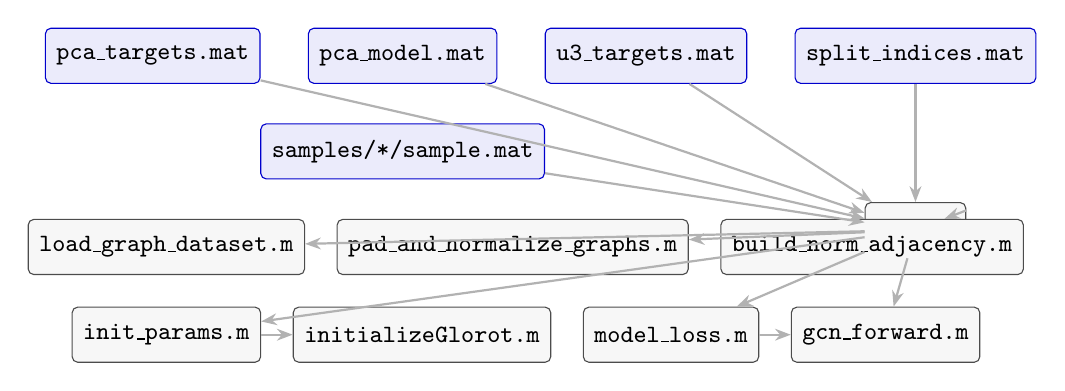
\begin{tikzpicture}[
  every node/.style={font=\ttfamily\small,align=center},
  arrow/.style={-{Stealth[length=2mm]},thick,draw=gray!60},
  box/.style={rectangle,draw=black!70,rounded corners=2pt,
              fill=codebg,inner sep=4pt,minimum height=7mm},
  data/.style={rectangle,draw=matlabblue,rounded corners=2pt,
               fill=matlabblue!8,inner sep=4pt,minimum height=7mm}
]

\node[data]  (pcat)  {pca\_targets.mat};
\node[data,right=6mm of pcat]  (pcam)  {pca\_model.mat};
\node[data,right=6mm of pcam]  (u3)    {u3\_targets.mat};
\node[data,right=6mm of u3]    (sidx)  {split\_indices.mat};
\node[data,below=5mm of pcam]  (samp)  {samples/*/sample.mat};

\node[box,below=15mm of sidx]  (main)  {Main.m};

\node[box,below=5mm of samp,xshift=-30mm]  (load)  {load\_graph\_dataset.m};
\node[box,right=4mm of load]               (pad)   {pad\_and\_normalize\_graphs.m};
\node[box,right=4mm of pad]                (adj)   {build\_norm\_adjacency.m};

\node[box,below=4mm of load]  (init)  {init\_params.m};
\node[box,right=4mm of init]  (glo)   {initializeGlorot.m};
\node[box,right=4mm of glo]   (loss)  {model\_loss.m};
\node[box,right=4mm of loss]  (fwd)   {gcn\_forward.m};

\foreach \f in {pcat,pcam,u3,sidx,samp} { \draw[arrow] (\f) -- (main); }
\draw[arrow] (main) -- (load);
\draw[arrow] (main) -- (pad);
\draw[arrow] (main) -- (adj);
\draw[arrow] (main) -- (init);
\draw[arrow] (main) -- (loss);
\draw[arrow] (main) -- (fwd);
\draw[arrow] (init) -- (glo);
\draw[arrow] (loss) -- (fwd);

\end{tikzpicture}
\end{center}

Blue boxes are data artifacts; grey boxes are code.

\section{Walkthrough of one complete training step}

For concreteness, here is what happens in a single call to
\texttt{dlfeval(lossfcn, \ldots)} for a batch of $32$ graphs.

\begin{enumerate}[leftmargin=1.4em]
  \item \textbf{Inputs are sliced on the CPU.}
        \texttt{X\_pad(:,:,idx)}, \texttt{A\_hat(idx)},
        \texttt{M(:,:,idx)}, and \texttt{Z\_target(:,:,idx)} all select the
        batch dimension. None of these is a \texttt{dlarray} yet.
  \item \textbf{\texttt{dlfeval} enters tracing mode.}
        Inside the traced call, any math involving \texttt{params} (which
        are \texttt{dlarray}s) produces intermediate \texttt{dlarray}s that
        record their history.
  \item \textbf{Embedding.}
        \texttt{u = tanh(pagemtimes(W\_emb, X) + b\_emb)}
        produces \texttt{u} of shape $64\times 300\times 32$ as a
        \texttt{dlarray}.
  \item \textbf{Three residual GCN layers.}
        Each layer first does a batched $Wu$ with \texttt{pagemtimes}, then
        loops over the $32$ graphs to apply its sparse $\hat A$ from the
        left (dense $\hat A\cdot v^{\!\top}$ each), transposes back, adds
        the residual and a \texttt{tanh} correction.
  \item \textbf{Masked mean-pool.}
        \texttt{sum(u .* mask, 2) ./ sum(mask, 2)} reduces the node
        dimension to $1$, yielding a $64\times 1\times 32$ graph
        embedding.
  \item \textbf{Pool MLP + decoder.}
        \texttt{pagemtimes(W\_pool, h)} followed by \texttt{tanh}, then
        \texttt{pagemtimes(W\_dec, h)} yields the standardized PCA
        prediction $\widehat Z$ of shape $8\times 1\times 32$.
  \item \textbf{Loss.}
        \texttt{loss = mean((Zhat - Z\_target).\^{}2, "all")} is a
        scalar \texttt{dlarray}.
  \item \textbf{Gradient.}
        \texttt{grad = dlgradient(loss, params)} walks the recorded
        computation graph backward and returns a struct of gradients with
        the same field structure as \texttt{params}.
  \item \textbf{Weight decay.}
        \texttt{grad = dlupdate(@(g,p) g + wd*p, grad, params)} adds
        $\lambda W$ to each gradient.
  \item \textbf{Adam step.}
        \texttt{[params, avgG, avgSqG] = adamupdate(\ldots)} applies the
        update and returns new running averages.
  \item \textbf{Scalar logging.}
        \texttt{gather(extractdata(loss))} exits both the autograd and GPU
        wrappers so \texttt{epochLoss} can accumulate in a plain
        \texttt{double}.
\end{enumerate}

\section{Suggested experiments for intuition}

\begin{itemize}
  \item Set $K=1$ vs.\ $K=5$. Deeper models begin to over-smooth; the
        validation loss should reach its floor somewhere in between.
  \item Remove the residual
        (\texttt{u = tanh(Vagg)} instead of \texttt{u = u + tanh(Vagg)})
        and watch training destabilize for $K\geq 3$.
  \item Swap the masked mean-pool for a sum-pool
        (remove the \texttt{./ sum(mask,2)}) and observe the blow-up in
        the loss scale.
  \item Set \texttt{weight\_decay = 0} and watch the gap between training
        and validation loss widen.
  \item Print \texttt{size(u)} inside \texttt{gcn\_forward} at each layer
        to verify the shape tracking against the table above.
\end{itemize}

\appendix

\section{Full \texttt{Main.m}}

The helpers are reproduced inline throughout the document. The top-level
script \texttt{Matlab/GNN/models/Main.m} is given here in full for
reference.

\begin{lstlisting}[caption={\texttt{models/Main.m}}]
%% GNN to predict spinodoid sheet deformation (8-dim PCA target)

clear; close all; clc;
rng(1);

scriptDir = fileparts(mfilename('fullpath'));   % .../Matlab/GNN/models
gnnRoot   = fileparts(scriptDir);              % .../Matlab/GNN
addpath(genpath(fullfile(gnnRoot, 'helpers')));

%% Config

training     = true;
K            = 3;       % GCN layers
hiddenDim    = 64;
poolDim      = 64;
batchSize    = 32;
maxEpochs    = 120;
lr0          = 3e-3;
decay_rate   = 0.99;
weight_decay = 1e-5;
valFreq      = 2;
patience     = 10;
minDelta     = 1e-4;
gpuUse       = canUseGPU;

targetsDir = fullfile(gnnRoot, 'data', 'dataset', 'targets');
samplesDir = fullfile(gnnRoot, 'data', 'dataset', 'samples');
bestDir    = fullfile(scriptDir, 'best');
if ~isfolder(bestDir), mkdir(bestDir); end

paramFile    = fullfile(bestDir, 'best_params.mat');
progressFile = fullfile(bestDir, 'training_log.mat');

%% Load targets

t = load(fullfile(targetsDir, 'pca_targets.mat'), ...
    'Z_train', 'Z_val', 'Z_test', 'train_ids', 'val_ids', 'test_ids', 'n_components');
p = load(fullfile(targetsDir, 'pca_model.mat'),   'coeff', 'u3_mean', 's_grid');
u = load(fullfile(targetsDir, 'u3_targets.mat'),  'U3_mat');
sp = load(fullfile(targetsDir, 'split_indices.mat'), 'val_idx');

Z_train   = t.Z_train;    % n_train x nComp
Z_val     = t.Z_val;
Z_test    = t.Z_test;
train_ids = t.train_ids;
val_ids   = t.val_ids;
test_ids  = t.test_ids;
nComp     = t.n_components;

coeff   = p.coeff;     % N_GRID x nComp
u3_mean = p.u3_mean;   % 1 x N_GRID
s_grid  = p.s_grid;

U3_mat  = u.U3_mat;
val_idx = sp.val_idx;

nTrain = numel(train_ids);
nVal   = numel(val_ids);
nTest  = numel(test_ids);

%% Load graphs

fprintf('Loading %d training graphs...\n',   nTrain);
[Xtr, eiTr, NTr] = load_graph_dataset(train_ids, samplesDir);
fprintf('Loading %d validation graphs...\n', nVal);
[Xvl, eiVl, NVl] = load_graph_dataset(val_ids, samplesDir);
fprintf('Loading %d test graphs...\n',       nTest);
[Xts, eiTs, NTs] = load_graph_dataset(test_ids, samplesDir);

allX  = [Xtr;  Xvl;  Xts];
allEI = [eiTr; eiVl; eiTs];
allN  = [NTr;  NVl;  NTs];
nAll  = nTrain + nVal + nTest;

trainLocal = (1 : nTrain)';
valLocal   = (nTrain+1       : nTrain+nVal)';
testLocal  = (nTrain+nVal+1  : nAll)';

%% Normalize features & build adjacency

trainMask = false(nAll, 1);
trainMask(trainLocal) = true;

maxN = max(allN);
fprintf('maxN=%d  nAll=%d\n', maxN, nAll);

[X_pad, nodeMask, normStats] = pad_and_normalize_graphs(allX, allN, trainMask);
A_hat = build_norm_adjacency(allEI, allN, maxN);

%% Standardize PCA targets

Z_mean = mean(Z_train, 1);
Z_std  = std(Z_train, 0, 1);
Z_std(Z_std < 1e-8) = 1e-8;

normStats.Z_mean = Z_mean;
normStats.Z_std  = Z_std;

Z_all     = [Z_train; Z_val; Z_test];
Z_all_std = (Z_all - Z_mean) ./ Z_std;
Z_target  = single(reshape(Z_all_std', nComp, 1, []));

%% Initialize model

F      = 3;
params = init_params(F, hiddenDim, poolDim, nComp, K);

%% Training

M = single(nodeMask);

if training
    lossfcn = dlaccelerate(@model_loss);
    clearCache(lossfcn);

    avgG = []; avgSqG = []; iteration = 0;
    bestValLoss = inf; best_params = params;
    bestEpoch = 0; noImproveCount = 0;

    train_losses = zeros(maxEpochs, 1);
    val_losses   = zeros(maxEpochs, 1);

    numIters = max(1, ceil(nTrain / batchSize));

    tic
    for epoch = 1:maxEpochs
        lr   = lr0 * decay_rate^(epoch - 1);
        perm = trainLocal(randperm(nTrain));
        epochLoss = 0;

        for b = 1:numIters
            si  = (b-1)*batchSize + 1;
            ei  = min(b*batchSize, nTrain);
            idx = perm(si:ei);

            [loss, grad] = dlfeval(lossfcn, params, ...
                X_pad(:,:,idx), A_hat(idx), K, M(:,:,idx), gpuUse, Z_target(:,:,idx));

            grad      = dlupdate(@(g,p) g + weight_decay*p, grad, params);
            iteration = iteration + 1;
            [params, avgG, avgSqG] = adamupdate(params, grad, avgG, avgSqG, iteration, lr);

            epochLoss = epochLoss + double(gather(extractdata(loss)));
        end

        train_losses(epoch) = epochLoss / numIters;

        if epoch == 1 || mod(epoch, valFreq) == 0
            [valLoss, ~] = dlfeval(lossfcn, params, ...
                X_pad(:,:,valLocal), A_hat(valLocal), K, ...
                M(:,:,valLocal), gpuUse, Z_target(:,:,valLocal));
            valLoss = double(gather(extractdata(valLoss)));
            val_losses(epoch) = valLoss;

            if valLoss < bestValLoss - minDelta
                bestValLoss = valLoss;
                best_params = params;
                bestEpoch   = epoch;
                noImproveCount = 0;
            else
                noImproveCount = noImproveCount + 1;
            end

            if noImproveCount >= patience
                break;
            end
        end

        if mod(epoch, 2) == 0 || epoch == 1
            save(progressFile, 'epoch', 'train_losses', 'val_losses', 'params', '-v7.3');
        end
    end
    toc

    params = best_params;
    cfg = struct('K', K, 'hiddenDim', hiddenDim, 'poolDim', poolDim, ...
                 'batchSize', batchSize, 'lr0', lr0, 'maxEpochs', maxEpochs, ...
                 'bestEpoch', bestEpoch, 'nComp', nComp);
    save(paramFile, 'params', 'cfg', 'normStats', 'train_losses', 'val_losses');

else
    load(paramFile, 'params', 'cfg', 'normStats', 'train_losses', 'val_losses');
end

%% Evaluate on validation set

Zhat_std = gcn_forward(params, X_pad(:,:,valLocal), A_hat(valLocal), K, M(:,:,valLocal), gpuUse);
Zhat_std = gather(extractdata(Zhat_std));
Zhat_val = squeeze(Zhat_std).' .* Z_std + Z_mean;

err_z  = Zhat_val - Z_val;
mse_z  = mean(err_z(:).^2);
R2_z   = 1 - sum(err_z(:).^2) / sum((Z_val(:) - mean(Z_val(:))).^2);

U3_pred = Zhat_val * coeff' + u3_mean;
U3_true = U3_mat(val_idx, :);
err_u3  = U3_pred - U3_true;
mse_u3  = mean(err_u3(:).^2);
R2_u3   = 1 - sum(err_u3(:).^2) / sum((U3_true(:) - mean(U3_true(:))).^2);

fprintf('Validation Z-space:  MSE=%.4g  R2=%.4f\n', mse_z, R2_z);
fprintf('Validation u3-space: MSE=%.4g  R2=%.4f\n', mse_u3, R2_u3);
\end{lstlisting}

\end{document}
